\lecture{12}{Paramagnetism}{Qiang Zhu}{scribe-name1,2,3}

\section{Two-state paramagnet}
The system consists of $N$ spin particles, immersed in a constant magnetic field $B$ point in the z direction. Each particle behaves like a compass needle (\textbf{dipoles}). According to quantum mechanics, the component of a particle's dipole moment will take quantized value (see Fig. \ref{fig1}). 

\begin{figure}[h]
\centering
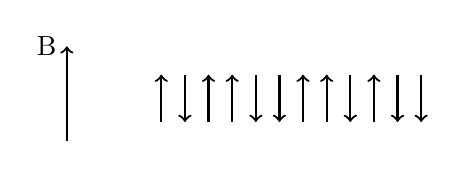
\begin{tikzpicture}[thick, scale=0.6]
\draw[->] (1.0,0.4)  -- (1.0,1.4) ;
\draw[->] (1.5,1.4)  -- (1.5,0.4) ;
\draw[->] (2.0,0.4)  -- (2.0,1.4) ;
\draw[->] (2.5,0.4)  -- (2.5,1.4) ;
\draw[->] (3.0,1.4)  -- (3.0,0.4) ;
\draw[->] (3.5,1.4)  -- (3.5,0.4) ;
\draw[->] (4.0,0.4)  -- (4.0,1.4) ;
\draw[->] (4.5,0.4)  -- (4.5,1.4) ;
\draw[->] (5.0,1.4)  -- (5.0,0.4) ;
\draw[->] (5.5,0.4)  -- (5.5,1.4) ;
\draw[->] (6.0,1.4)  -- (6.0,0.4) ;
\draw[->] (6.5,1.4)  -- (6.5,0.4) ;
\draw[->] (-1.0,0) -- (-1.0,2) node [left]{B};

\end{tikzpicture}
\caption{A two-state paramagnet with an external magnetic field B and N microscopic magnetic dipoles facing up and down. The energy level of a single dipole in an
ideal two-state paramagent are -$\mu$B for the up date and $\mu$B for the down state.}
\label{fig1}

\end{figure}

The total energy of the system is
\begin{equation} \label{eq1} 
U = \mu B(N_{\downarrow} - N_{\uparrow}) = \mu B(N-2N_{\uparrow})
\end{equation}

Where $N_{\uparrow}$ and $N_{\downarrow}$ are the number of up and down dipoles, and $N$ is the total number. Due the distribution of $N_{\uparrow}$ and $N_{\downarrow}$ , the total state may exhibit \textbf{magnetization}, $M$, which is the total magnetic moment of the whole system. Each up dipole has +$\mu$ and each down has -$\mu$. So,
\begin{equation}
    M = \mu(N_{\uparrow} - N_{\downarrow}) = -\frac{U}{B}
\end{equation}

Our goal is to understand how $U$ and $M$ relate to the temperature. Therefore, we need to know the multiplicity (since we know $T$ is related to the entropy).
\begin{equation}
    \Omega(N_{\uparrow}) = \binom{N}{N_{\uparrow}} = \frac{N!}{N_{\uparrow}N_{\downarrow}}.
\end{equation}

\section{Numerical results}

We can draw the the $\Omega$-U diagram. Clearly, the maximum of $\Omega$ can be achieved when $N_{\uparrow}$ = $N_{\uparrow}$. Namely, $U$ is zero.
\begin{enumerate}
    \item When all dipoles are pointing up, $U$ reaches the minimum, and the slope goes very large. 
    \item When $\Omega$ reaches the maximum, the slope goes zeros, and then switch the sign.
\end{enumerate}

Since we know that $T$ is the reciprocal of the slope of $S-U$ graph, it means that the temperature is actually infinite when $U=0$. That is to say, the system will gladly give up energy to any other system whose temperature is finite. At higher energies, the slope becomes negative. Does it mean temperture becomes negative??

Negative temperature can occur only for a system whose total energy is limited, so that the multiplicity decreases as the maximum allowed energy is approached. 


\begin{figure}[ht]
    \centering
    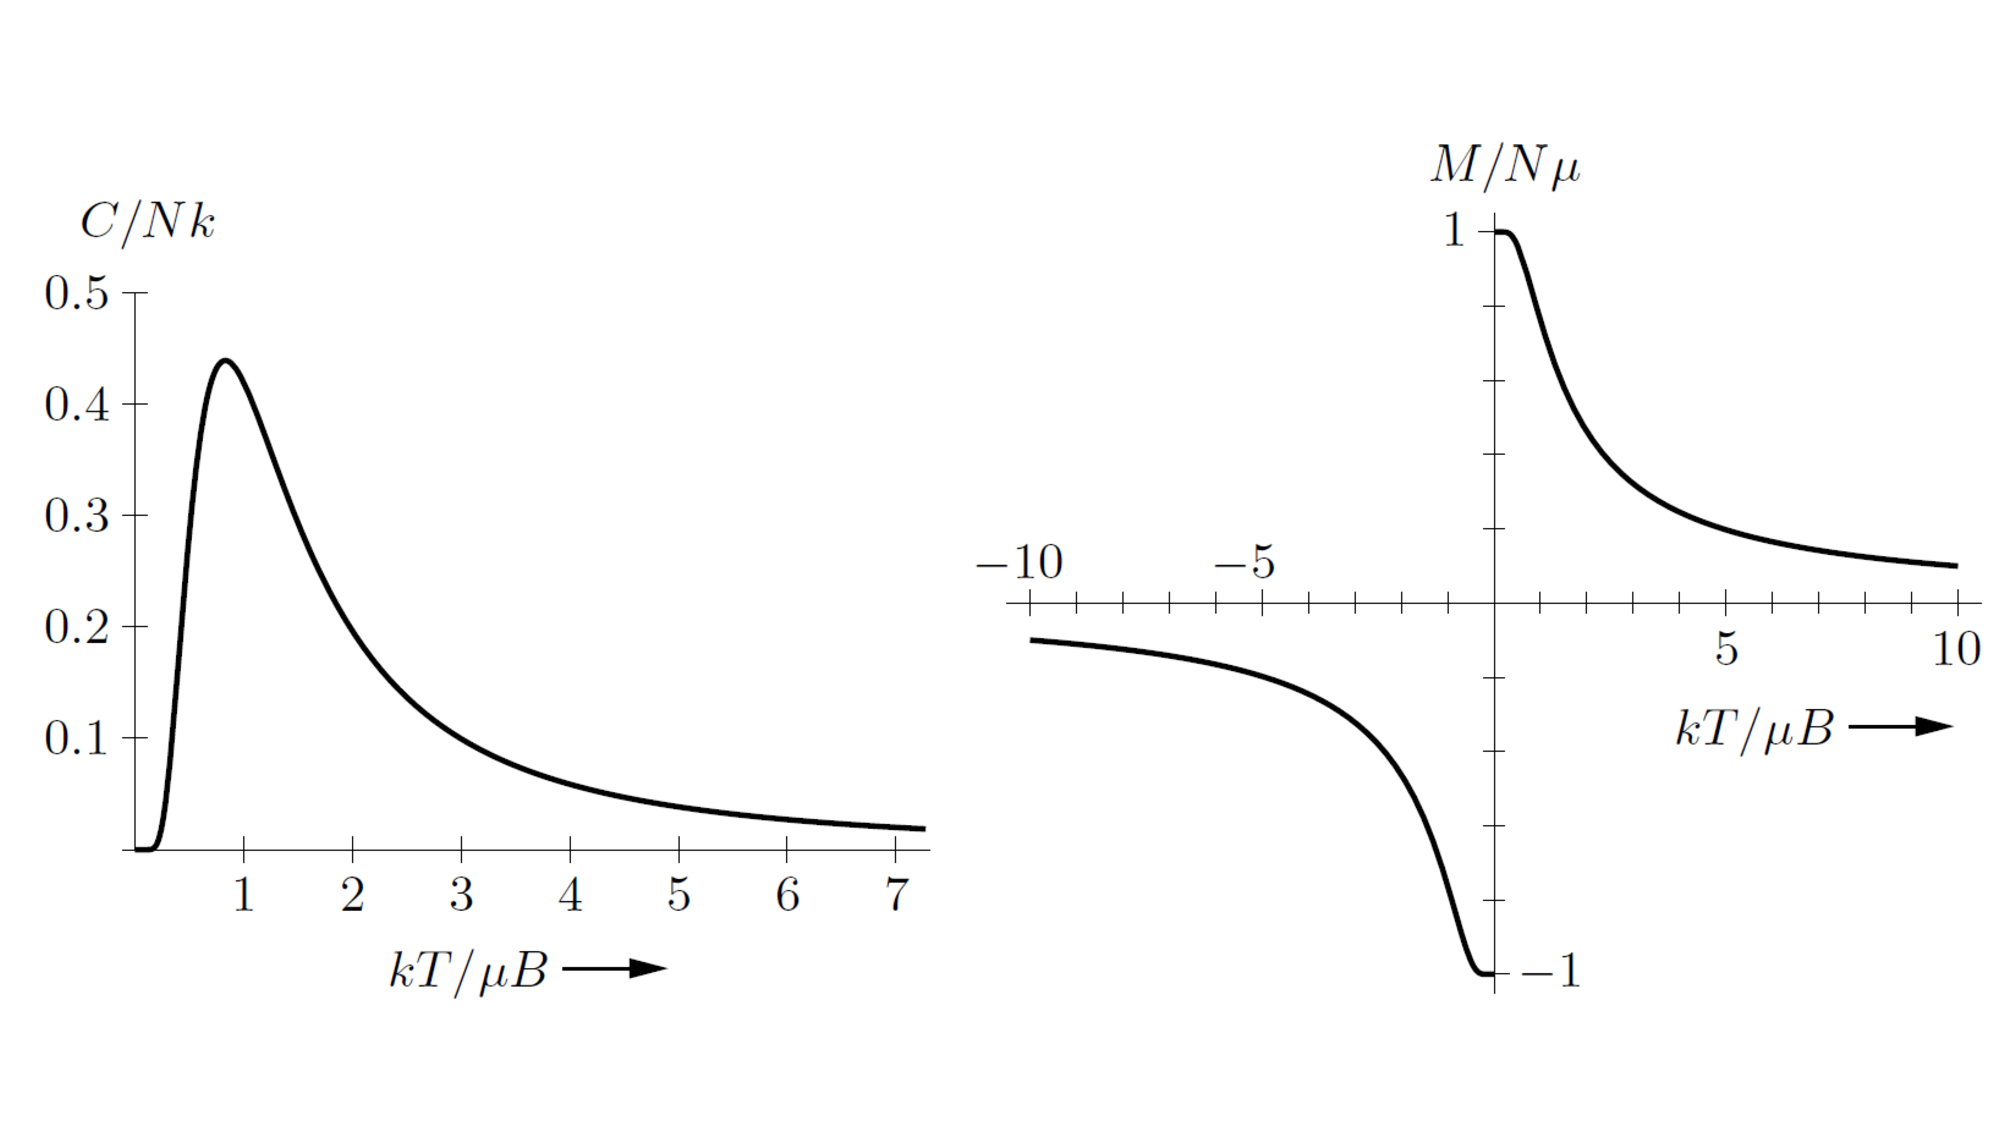
\includegraphics[width=0.9\linewidth]{imgs/Magnetic.pdf}
    \caption{Heat capacity and magnetization of a two-state paramagnet (computed
from the analytic formulas derived later in the text). Copyright 2000,
Addison-Wesley.}
    \label{fig:results}
\end{figure}

\section{Analytic solution}
We can also use the Stirling approximation to understand it analytically.
\begin{equation} 
\begin{split}
    S/k & = \ln N! - \ln N_\uparrow ! - \ln (N-N_\uparrow)! \\
        & \approx \ln N - N - N_\uparrow \ln N_\uparrow + N_\uparrow - (N-N_\uparrow)\ln(N-N_\uparrow) + (N-N_\uparrow) \\
        & = N\ln N - N_\uparrow \ln N_\uparrow - (N-N_\uparrow) \ln(N-N_\uparrow)
\end{split}
\end{equation}

To find the temperature relation, we need to differentiate $S$ with respect to $U$.
\begin{equation}
 \frac{1}{T} = \bigg(\frac{\partial S}{\partial U}\bigg)_{N, B} 
             = \frac{\partial N_\uparrow}{\partial U} \frac{\partial S}{\partial N_\uparrow} 
             = -\frac{1}{2\mu B}\frac{\partial S}{\partial N_\uparrow}    
\end{equation}
Now we get
\begin{equation}
    \frac{1}{T} = \frac{k}{2\mu B} \ln \frac{N-U/\mu B}{N+U/\mu B}
\end{equation}

Therefore, 
\begin{equation}
    U = N\mu B\frac{1-e^{2\mu B/kT}}{1+e^{2\mu B/kT}} = -N\mu B\tanh \bigg({\frac{\mu B}{kT}}\bigg)
\end{equation}
and the magnetization is
\begin{equation}
    M = N\mu\tanh \bigg({\frac{\mu B}{kT}}\bigg)
\end{equation}



To calculate the heat capacity of the paramagnet, we just need to differentiate the equation with respect to $T$;
\begin{equation}
    C_B = \bigg(\frac{\partial U}{\partial T}\bigg)_{N, B} = Nk \frac{(\mu B/kT)^2}{\cosh^2(\mu B/kT)}
\end{equation}
This function approaches zero at both high T and low T. 

At room temperature $\mu B = 5.8 \times 10^{-5}$ eV, while $kT$ is about 1/40 eV. So, we can assume that $\mu B/kT \ll 1$. In this limit, $\tanh(x) \approx x$, so the magnetization becomes 
\begin{equation}
    M \approx \frac{N\mu^2B}{kT}
\end{equation}

The face that $M \propto 1/T$ was discovered by Pierre Curie and is known as \textbf{Curie's law}. 


\section{Homework}
Problem 3.19, 3.22, 3.23
